% ===== map =====
\section*{Maximum a Posteriori (MAP)}
% ---- CS189 scope checklist: must include ([x] = already covered) ----
% Source: Lectures 5, 7; reference sheet pp.3-4
% [ ] Bayes' theorem: posterior is proportional to likelihood x prior; p(D) drops out
% [ ] MAP = argmax [ sum ln p(t_n | x_n, w) + ln p(w) ]
% [ ] Coin with a Beta(a, b) prior: mu_MAP = (n_1 + a - 1) / (N + a + b - 2)
% [ ] Small N: the prior wins; large N: MAP -> MLE
% [ ] The prior acts as a regularizer (Gaussian prior -> ridge, Laplace prior -> lasso)
% ----

\subsection*{Why MAP?}
MLE uses only the data, so a small sample gives overconfident estimates. For example, flip a coin twice and get two heads: $\theta_{\text{ML}} = \tfrac{2}{2} = 1$, so the model says tails can never happen.

MAP fixes this by adding a \textbf{prior}: a distribution $p(\theta)$ describing what we believe about $\theta$ before seeing any data (e.g.\ ``the coin is probably close to fair'').

\subsection*{Bayes' Theorem for the Parameter}
\begin{keeptogether}
MLE treats $\theta$ as a fixed unknown number. MAP treats $\theta$ as a random variable and updates its distribution with Bayes' theorem:
\[
\underbrace{p(\theta \mid \mathcal{D})}_{\makebox[0pt]{\scriptsize posterior}}
= \frac{\overbrace{p(\mathcal{D} \mid \theta)}^{\makebox[0pt]{\scriptsize likelihood}}\;\overbrace{p(\theta)}^{\makebox[0pt]{\scriptsize prior}}}{p(\mathcal{D})}
\]
The posterior combines the two sources of information:
\begin{itemize}
  \item \textbf{Prior} $p(\theta)$: the belief about $\theta$ before seeing data.
  \item \textbf{Likelihood} $p(\mathcal{D} \mid \theta)$: the same quantity MLE maximizes.
  \item \textbf{Posterior} $p(\theta \mid \mathcal{D})$: the updated belief after seeing the data.
\end{itemize}
\end{keeptogether}

\begin{keeptogether}
MAP picks the peak of the posterior. The denominator $p(\mathcal{D})$ does not depend on $\theta$, so it does not move the peak and drops out:
\[
\theta_{\text{MAP}} = \arg\max_{\theta}\; p(\mathcal{D} \mid \theta)\, p(\theta) = \arg\max_{\theta} \big[\underbrace{\ln p(\mathcal{D} \mid \theta)}_{\makebox[0pt]{\scriptsize same as MLE}} + \underbrace{\ln p(\theta)}_{\makebox[0pt]{\scriptsize prior}}\big]
\]
\textbf{Big idea:} MAP is MLE with one extra term, $\ln p(\theta)$, that pulls the estimate toward what the prior believes. For a coin with 3 heads in 4 flips and a prior that it is probably fair:

{\centering
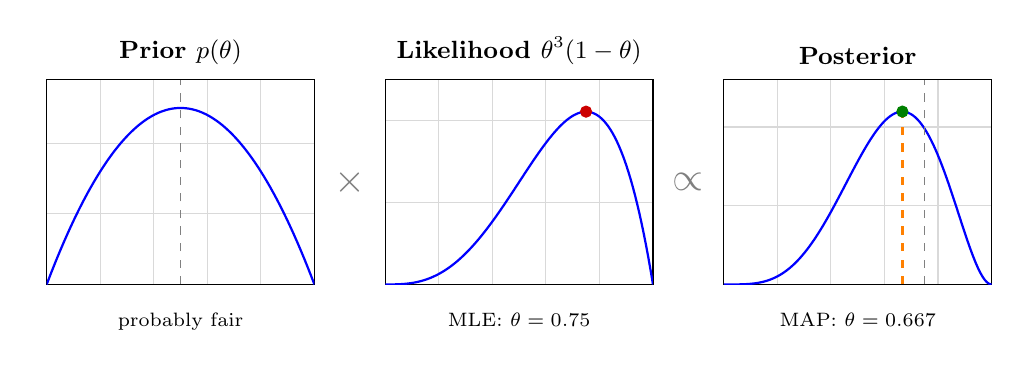
\begin{tikzpicture}
\begin{axis}[name=pr, scale only axis, width=3.4cm, height=2.6cm,
    xmin=0, xmax=1, ymin=0, ymax=0.29, enlargelimits=false,
    grid=major, grid style={gray!30}, major tick length=0pt,
    xticklabels={}, yticklabels={},
    title={\small\textbf{Prior $p(\theta)$}}, title style={yshift=-4pt},
    xlabel={\scriptsize probably fair}, label style={font=\scriptsize}]
\addplot[thick, blue, domain=0:1, samples=80] {x*(1-x)};
\addplot[gray, dashed] coordinates {(0.5,0) (0.5,0.29)};
\end{axis}
\node[font=\Large, gray, xshift=0.45cm] at (pr.east) {$\times$};
\begin{axis}[name=lk, at={(pr.east)}, anchor=west, xshift=0.9cm, scale only axis, width=3.4cm, height=2.6cm,
    xmin=0, xmax=1, ymin=0, ymax=0.125, enlargelimits=false,
    grid=major, grid style={gray!30}, major tick length=0pt,
    xticklabels={}, yticklabels={},
    title={\small\textbf{Likelihood $\theta^3(1-\theta)$}}, title style={yshift=-4pt},
    xlabel={\scriptsize MLE: $\theta = 0.75$}, label style={font=\scriptsize}]
\addplot[thick, blue, domain=0:1, samples=120] {x^3*(1-x)};
\addplot[only marks, mark=*, red!80!black, mark size=2pt] coordinates {(0.75,0.1055)};
\end{axis}
\node[font=\Large, gray, xshift=0.45cm] at (lk.east) {$\propto$};
\begin{axis}[name=po, at={(lk.east)}, anchor=west, xshift=0.9cm, scale only axis, width=3.4cm, height=2.6cm,
    xmin=0, xmax=1, ymin=0, ymax=0.026, enlargelimits=false, scaled y ticks=false,
    grid=major, grid style={gray!30}, major tick length=0pt,
    xticklabels={}, yticklabels={},
    title={\small\textbf{Posterior}}, title style={yshift=-4pt},
    xlabel={\scriptsize MAP: $\theta = 0.667$}, label style={font=\scriptsize}]
\addplot[thick, blue, domain=0:1, samples=120] {x^4*(1-x)^2};
\addplot[gray, dashed] coordinates {(0.75,0) (0.75,0.026)};
\addplot[orange, dashed, thick] coordinates {(0.667,0) (0.667,0.02195)};
\addplot[only marks, mark=*, green!50!black, mark size=2pt] coordinates {(0.667,0.02195)};
\end{axis}
\end{tikzpicture}
\par}
{\centering\scriptsize The prior pulls the estimate from the MLE $0.75$ (gray dashed) toward $0.5$, to $0.667$.\par}
\end{keeptogether}


\subsection*{Choosing a Prior: the Beta Distribution}
\begin{keeptogether}
A common prior for a probability $\theta \in [0, 1]$ is the \textbf{Beta} distribution, with parameters $a, b > 0$:
\[
p(\theta) \;\propto\; \theta^{\,a-1}(1-\theta)^{\,b-1}
\]
With $a = b$, the prior is centered at $0.5$, and larger values express a stronger belief that the coin is fair:

{\centering
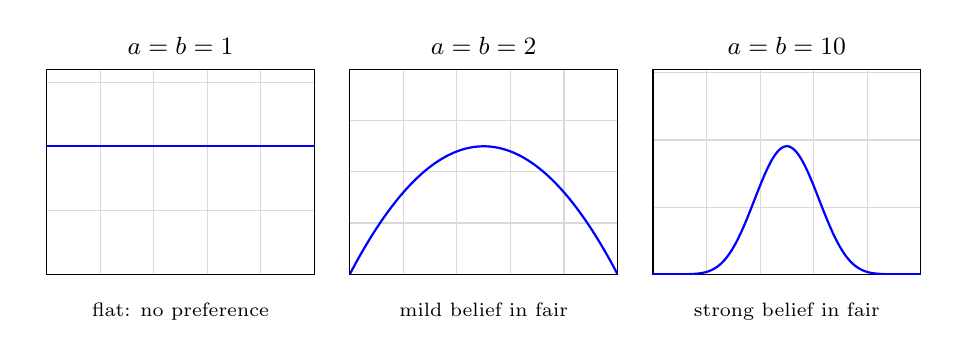
\begin{tikzpicture}
\begin{axis}[name=b1, scale only axis, width=3.4cm, height=2.6cm,
    xmin=0, xmax=1, ymin=0, ymax=1.6, enlargelimits=false,
    grid=major, grid style={gray!30}, major tick length=0pt,
    xticklabels={}, yticklabels={},
    title={\small\textbf{$a = b = 1$}}, title style={yshift=-4pt},
    xlabel={\scriptsize flat: no preference}, label style={font=\scriptsize}]
\addplot[thick, blue, domain=0:1, samples=2] {1};
\end{axis}
\begin{axis}[name=b2, at={(b1.east)}, anchor=west, xshift=0.45cm, scale only axis, width=3.4cm, height=2.6cm,
    xmin=0, xmax=1, ymin=0, ymax=0.4, enlargelimits=false,
    grid=major, grid style={gray!30}, major tick length=0pt,
    xticklabels={}, yticklabels={},
    title={\small\textbf{$a = b = 2$}}, title style={yshift=-4pt},
    xlabel={\scriptsize mild belief in fair}, label style={font=\scriptsize}]
\addplot[thick, blue, domain=0:1, samples=80] {x*(1-x)};
\end{axis}
\begin{axis}[name=b3, at={(b2.east)}, anchor=west, xshift=0.45cm, scale only axis, width=3.4cm, height=2.6cm,
    xmin=0, xmax=1, ymin=0, ymax=6.1e-6, enlargelimits=false, scaled y ticks=false,
    grid=major, grid style={gray!30}, major tick length=0pt,
    xticklabels={}, yticklabels={},
    title={\small\textbf{$a = b = 10$}}, title style={yshift=-4pt},
    xlabel={\scriptsize strong belief in fair}, label style={font=\scriptsize}]
\addplot[thick, blue, domain=0:1, samples=120] {x^9*(1-x)^9};
\end{axis}
\end{tikzpicture}
\par}
\end{keeptogether}

\subsection*{MAP for the Coin}
We follow the same three steps as MLE, now with the prior multiplied in. Data: $n_1$ heads and $n_0$ tails in $N$ flips.

\begin{keeptogether}
\textbf{Step 1: IID $\Rightarrow$ product.} Multiply the Bernoulli likelihood by the Beta prior and collect the powers:
\[
p(\theta \mid \mathcal{D}) \;\propto\; \underbrace{\theta^{\,n_1}(1-\theta)^{\,n_0}}_{\makebox[0pt]{\scriptsize likelihood}}\;\underbrace{\theta^{\,a-1}(1-\theta)^{\,b-1}}_{\makebox[0pt]{\scriptsize prior}} = \theta^{\,n_1+a-1}(1-\theta)^{\,n_0+b-1}
\]
The posterior is again a Beta distribution, with parameters $n_1 + a$ and $n_0 + b$. A prior with this property is called a \textbf{conjugate prior}.
\end{keeptogether}

\begin{keeptogether}
\textbf{Step 2: Log $\Rightarrow$ sum.}
\[
\ln p(\theta \mid \mathcal{D}) = (n_1 + a - 1)\ln\theta + (n_0 + b - 1)\ln(1-\theta) + \text{const}
\]
\end{keeptogether}

\begin{keeptogether}
\textbf{Step 3: Maximize the posterior.} This has the same form as the MLE objective $n_1 \ln\theta + n_0\ln(1-\theta)$, with $n_1$ replaced by $n_1 + a - 1$ and $n_0$ by $n_0 + b - 1$. So the answer has the same form as $\theta_{\text{ML}} = \tfrac{n_1}{N}$:
\[
\theta_{\text{MAP}} = \frac{n_1 + a - 1}{N + a + b - 2}
\qquad \text{coin } (a = b = 2,\ 7 \text{ heads in } 10)\text{:} \quad \frac{7 + 1}{10 + 2} = 0.667
\]
\end{keeptogether}

\begin{keeptogether}
The prior acts like \textbf{pseudo-counts}: $a - 1$ imaginary heads and $b - 1$ imaginary tails added to the data. With $a = b = 2$, this adds one of each:
\[
\theta_{\text{MAP}} = \frac{n_1 + 1}{N + 2}
\qquad \text{two heads in two flips:} \quad \frac{2 + 1}{2 + 2} = 0.75 \quad (\text{vs. } \theta_{\text{ML}} = 1)
\]
This is called \textbf{Laplace smoothing}. The estimate is never exactly 0 or 1, which matters for rare events.
\end{keeptogether}

\subsection*{MAP vs.\ MLE as $N$ Grows}
\begin{keeptogether}
The pseudo-counts are fixed, so their effect shrinks as the real data grows. With $a = b = 2$ and 70\% heads:

\begin{center}
\begin{tabular}{rccc}
\toprule
$N$ & heads $n_1$ & $\theta_{\text{ML}} = \tfrac{n_1}{N}$ & $\theta_{\text{MAP}} = \tfrac{n_1 + 1}{N + 2}$ \\
\midrule
10 & 7 & 0.7 & 0.667 \\
100 & 70 & 0.7 & 0.696 \\
1000 & 700 & 0.7 & 0.6996 \\
\bottomrule
\end{tabular}
\end{center}

With small $N$, the prior dominates and pulls the estimate toward $0.5$. With large $N$, the data dominates and \textbf{MAP converges to MLE}. This is why large-data settings, such as most deep learning, often use plain MLE.
\end{keeptogether}

\subsection*{MAP for Regression: Priors as Regularization}
\begin{keeptogether}
The same idea applies to the weights $\mathbf{w}$ of linear regression. A common prior is that each weight is small and centered at 0: $w_j \sim \mathcal{N}(0, \tau^2)$. Combined with Gaussian noise $\sigma^2$ on the targets, minimizing the negative log-posterior gives:
\[
\mathbf{w}_{\text{MAP}} = \arg\min_{\mathbf{w}} \Big[\underbrace{\tfrac{1}{2\sigma^2}\|\mathbf{t} - X\mathbf{w}\|^2}_{\makebox[0pt]{\scriptsize \ensuremath{-\ln} likelihood}} + \underbrace{\tfrac{1}{2\tau^2}\|\mathbf{w}\|^2}_{\makebox[0pt]{\scriptsize \ensuremath{-\ln} prior}}\Big]
\]
Multiplying by $\sigma^2$ does not move the minimum, and gives exactly the regularized loss from the Regularization section:
\[
\mathbf{w}_{\text{MAP}} = \arg\min_{\mathbf{w}} \Big[\tfrac{1}{2}\|\mathbf{t} - X\mathbf{w}\|^2 + \tfrac{\lambda}{2}\|\mathbf{w}\|^2\Big]
\qquad \lambda = \frac{\sigma^2}{\tau^2}
\]
\textbf{Big idea:} a Gaussian prior on the weights is the same as \textbf{ridge} ($L_2$) regularization. A smaller $\tau$ (stronger belief that the weights are near 0) means a larger $\lambda$.
\end{keeptogether}

\begin{keeptogether}
The shape of the prior decides the penalty. A Laplace prior has a sharp peak at 0 and gives the $L_1$ penalty $\lambda\|\mathbf{w}\|_1$, which is \textbf{lasso}:

{\centering
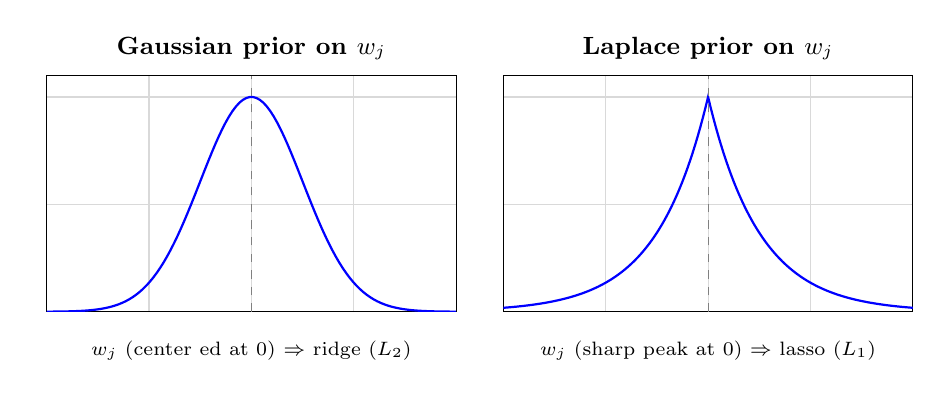
\begin{tikzpicture}
\begin{axis}[name=g, scale only axis, width=5.2cm, height=3cm,
    xmin=-4, xmax=4, ymin=0, ymax=1.1, enlargelimits=false,
    grid=major, grid style={gray!30}, major tick length=0pt,
    xticklabels={}, yticklabels={},
    title={\small\textbf{Gaussian prior on $w_j$}}, title style={yshift=-4pt},
    xlabel={\scriptsize $w_j$ (center   ed at 0) $\Rightarrow$ ridge ($L_2$)}, label style={font=\scriptsize}]
\addplot[thick, blue, domain=-4:4, samples=120] {exp(-x^2/2)};
\addplot[gray, dashed] coordinates {(0,0) (0,1.1)};
\end{axis}
\begin{axis}[name=l, at={(g.east)}, anchor=west, xshift=0.6cm, scale only axis, width=5.2cm, height=3cm,
    xmin=-4, xmax=4, ymin=0, ymax=1.1, enlargelimits=false,
    grid=major, grid style={gray!30}, major tick length=0pt,
    xticklabels={}, yticklabels={},
    title={\small\textbf{Laplace prior on $w_j$}}, title style={yshift=-4pt},
    xlabel={\scriptsize $w_j$ (sharp peak at 0) $\Rightarrow$ lasso ($L_1$)}, label style={font=\scriptsize}]
\addplot[thick, blue, domain=-4:4, samples=161] {exp(-abs(x))};
\addplot[gray, dashed] coordinates {(0,0) (0,1.1)};
\end{axis}
\end{tikzpicture}
\par}
\end{keeptogether}

So regularization is MAP estimation: the penalty term is the negative log of a prior that prefers small weights.